\documentclass[12pt]{article}

\usepackage[a4paper]{geometry}
\usepackage[utf8]{inputenc}
\usepackage[T1]{fontenc}
\usepackage[french]{babel}
\usepackage{graphicx}

\setcounter{tocdepth}{1}

\newcommand{\creerPage}[1]{
    \newpage
    \section{#1}
}

% \usetheme{Boadilla}

\title{Optimisation de circuits logiques}

\author{Alexandre JANNIAUX}

\begin{document}

    \maketitle
    \tableofcontents

    \newpage

    \creerPage{Représentation des circuits logiques}
        
        Circuit logique  / fonction combinatoire
            \begin{figure}[p]
                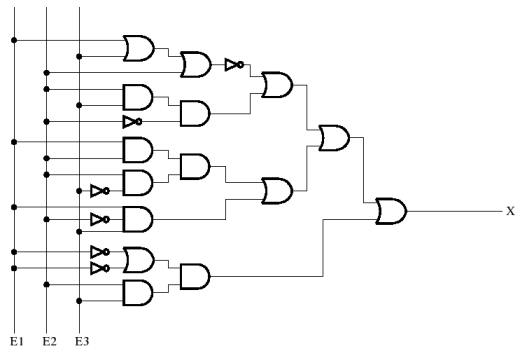
\includegraphics[width=8cm]{images/circuit_logique.png}
                \caption{Exemple de circuit logique}
                \label{fig:circ1}
            \end{figure}

        \[ \begin{aligned}
            f: \{0,1\}^3 &\longto &\{0,1\} \\
                (e_1,e_2,e_3) & \longmapsto & f(e_1,e_2,e_3) 
            \end{aligned}
        \]

        L'ensemble des fonctions combinatoires défini par induction

        MAIS : explosion combinatoire (algo naif)

    \creerPage{Méthode de Quine-McCluskey}

        \large{\textbf{Idée :}} Une fonction combinatoire est définie par le langage accepté (couverture).

        => On utilise l'algèbre de Boole pour simplifier les expressions

        \large{\textbf{Algorithme :}}
            \begin{enumerate}
                \item 
            \end{enumerate}
    \creerPage{Espresso}

\end{document}
